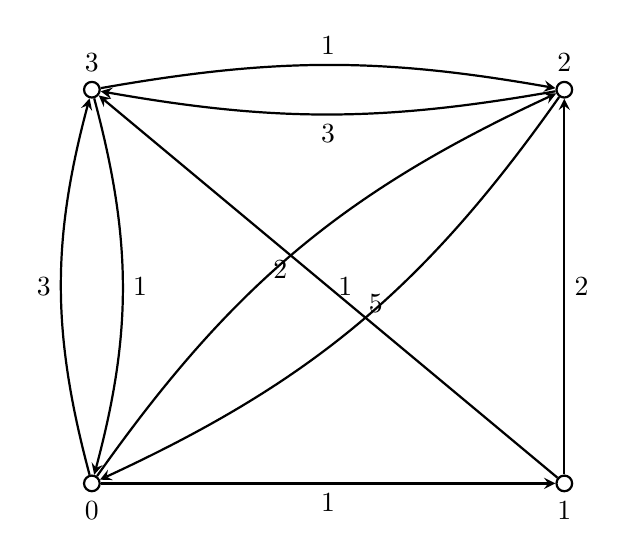
\begin{tikzpicture}
[nodedecorate/.style={shape=circle,inner sep=2pt,draw,thick},%
  arrowdecorate/.style={->,>=stealth,thick}]
% nodes or vertices
\node (0) at (0,0) [nodedecorate] {};
\node [below] at (0.south) {$0$};
\node (1) at (6,0) [nodedecorate] {};
\node [below] at (1.south) {$1$};
\node (2) at (6,5) [nodedecorate] {};
\node [above] at (2.north) {$2$};
\node (3) at (0,5) [nodedecorate] {};
\node [above] at (3.north) {$3$};
% edges or lines
\path
(0) edge[arrowdecorate] node[below]{$1$} (1)
(0) edge[arrowdecorate,bend left=15] node[below left]{$2$} (2)
(0) edge[arrowdecorate,bend left=15] node[left]{$3$} (3)
(1) edge[arrowdecorate] node[right]{$2$} (2)
(1) edge[arrowdecorate] node[right]{$1$} (3)
(2) edge[arrowdecorate,bend left=15] node[above right]{$5$} (0)
(2) edge[arrowdecorate,bend left=10] node[below]{$3$} (3)
(3) edge[arrowdecorate,bend left=15] node[right]{$1$} (0)
(3) edge[arrowdecorate,bend left=10] node[above]{$1$} (2);
\end{tikzpicture}
